Nervous systems in animals are different, from the simple ones found in insects to more complex ones in reptiles, birds and mammals. They are all mainly composed of a special kind of cell, the neuron, that excels at long distance communication. Most animal's nervous systems include an organ called the \emph{brain} which plays a central role on the everyday life of the animal. In most cases the brain will be located in the head which is the closest location to the primary sensing organs like eyes, tongue or ears~\cite{scholarpedia-brain}.\\


The \emph{human brain} is an exquisite piece of evidence of energy-efficient biological computation; the result of millions of years of an evolutionary process. It's been subject of multiple studies and, yet, we are barely getting to know it. The human brain consists of around $10^{12}$ individual cells called \emph{neurons} which are interconnected through about $10^{15}$ special structures known as \emph{synapses}.
%It can perform the most diverse activities, from bird spotting to mathematics to art. All of this with about 20 watts of energy spread across many small computational units called \emph{neurons}.
Studies have found that the brain is formed by many components, a brief description of the principal parts (shown in Figure \ref{fig:brain:components}) is presented next~\cite{thompson2000brain}. 
\begin{description}
  \item[Cerebrum], or \emph{cortex} is a wrinkled sheet of neurons that's the largest portion of the brain and is responsible of high level cognition, motor control, memory and problem solving, to name a few.
  \item[Cerebellum], also known as the ``small brain'' is mostly involved in sensorimotor tasks like balance or the coordination of the body.
  \item[Brain stem], which is located under the cerebrum and in front of the cerebellum, it connects the brain to the spinal cord and is in charge of automatic functions like breathing or digestion.
  \item[Limbic System], had been thought of as the ``old brain'' sits between the brain stem and the cortex. Some of its functions include hormonal control, emotions, learning and memory consolidation. 
\end{description}

\begin{figure}
  \begin{center}
    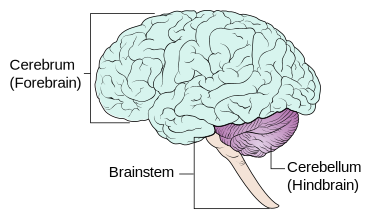
\includegraphics[width=0.8\textwidth]{Diagram_showing_some_of_the_main_areas_of_the_brain_CRUK_188}
    \caption{Main areas of the brain~\cite{wikipedia-images}.}
    \label{fig:brain:components}
  \end{center}
  
\end{figure}

About 80\% of the neurons in the brain are located inside the cortex. This thin sheet of about 1100 cm$^2$ area and a 2 to 4 mm. thickness is believed to be responsible for most of the high-level cognitive tasks humans can perform \textbf{CITE!!!}. The fact that is thoroughly wrinkled allows a larger area sheet, and neurons, to fit in the same volume. 
The cortex itself is composed of two symmetric shapes, the left and right \emph{hemispheres} (). Although both share functions, it has been observed that one hemisphere may dominate the other on some tasks~\cite{lateralization}. 



Measurements of the electrical activity in different areas of the cortex have led to the identification of areas that specialize on some tasks such as vision. 

So far, several functional units in the brain have been identified; but the exact mechanisms of how they perform is still unknown.


One of the most consuming tasks is vision, about 30\% of the cerebral cortex is used in visual perception. 

